%!TEX root = /Users/louis/Documents/PhD/Deliverables/Thesis/thesis.tex

\section{Analysis of Languages used for Migration}
\label{sec:analyis_of_languages_used_for_migration}
Section~\ref{subsec:co-evolution_categorisation} discussed existing approaches to model migration, highlighting variation in the languages used for specifying migration strategies. In this section, migration strategy languages are compared, using the example of metamodel evolution given in Section~\ref{subsec:co-evo_example}. From this comparison, requirements for a domain-specific language for specifying and executing model migration strategies are derived (Section~\ref{subsec:analysis}, and an implementation is described in the sequel. The work described in this section has been published in \cite{rose10flock}.

\subsection{Co-Evolution Example}
\label{subsec:co-evo_example}
Throughout this section, the following example of an evolution of a Petri net metamodel is used to discuss co-evolution and model migration. The same example has been used previously in co-evolution literature \cite{cicchetti08automating,garces09managing,wachsmuth07metamodel}.

\begin{figure}[bp]
	\centering
	\subfigure[Original metamodel.]
	{
	    \label{fig:original_mm}
	    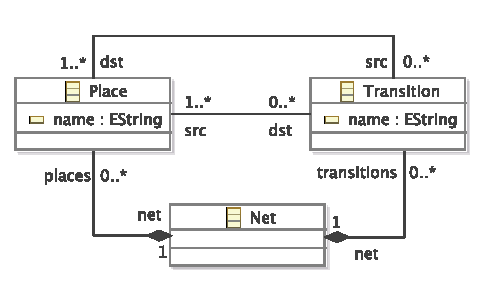
\includegraphics[width=4.75cm]{5.Implementation/images/petri_nets_before.pdf}
	}
	\subfigure[Evolved metamodel.]
	{
	    \label{fig:evolved_mm}
	    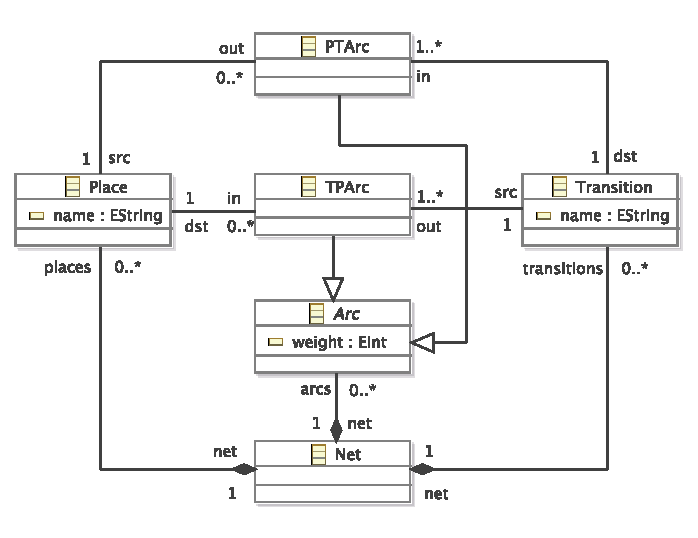
\includegraphics[width=6.25cm]{5.Implementation/images/petri_nets_after.pdf}
	}
	\caption[Exemplar metamodel evolution (Petri nets)]{Exemplar metamodel evolution. Taken from \cite{rose10flock}.}
\label{fig:petri_nets_mms}
\end{figure}

In Figure~\ref{fig:original_mm}, a Petri \texttt{Net} comprises \texttt{Place}s and \texttt{Transition}s. A \texttt{Place} has any number of \texttt{src} or \texttt{dst} \texttt{Transition}s. Similarly, a \texttt{Transition} has at least one \texttt{src} and \texttt{dst} \texttt{Place}. In this example, the metamodel in Figure~\ref{fig:original_mm} is to be evolved so as to support weighted connections between \texttt{Place}s and \texttt{Transition}s and between \texttt{Transition}s and \texttt{Place}s.

The evolved metamodel is shown in Figure~\ref{fig:evolved_mm}. \texttt{Place}s are connected to \texttt{Transition}s via instances of \texttt{PTArc}. Likewise, \texttt{Transition}s are connected to \texttt{Place}s via \texttt{TPArc}. Both \texttt{PTArc} and \texttt{TPArc} inherit from \texttt{Arc}, and therefore can be used to specify a \texttt{weight}.

Models that conformed to the original metamodel might not conform to the evolved metamodel. The following strategy can be used to migrate models from the original to the evolved metamodel:

\begin{enumerate}
	\item For every instance, t, of \texttt{Transition}: 
	\subitem For every \texttt{Place}, s, referenced by the \texttt{src} feature of t: 
	\subsubitem Create a new instance, arc, of \texttt{PTArc}. 
	\subsubitem Set s as the \texttt{src} of arc. 
	\subsubitem Set t as the \texttt{dst} of arc. 
	\subsubitem Add arc to the \texttt{arcs} reference of the \texttt{Net} referenced by t.
	
	\subitem For every \texttt{Place}, d, referenced by the \texttt{dst} feature of t: 
	\subsubitem Create a new instance, arc, of \texttt{TPArc}. 
	\subsubitem Set t as the \texttt{src} of arc. 
	\subsubitem Set d as the \texttt{dst} of arc. 
	\subsubitem Add arc to the \texttt{arcs} reference of the \texttt{Net} referenced by t.
	
	\item And nothing else changes.
\end{enumerate}

Using the above example, the existing approaches for specifying and executing model migration strategies are now compared.


\subsection{Existing Approaches}
\label{subsec:existing_migration_languages}
Using the above example, the existing approaches for specifying and executing model migration strategies are now compared. From this comparison, the strengths and weakness of each approach are highlighted and requirements for a model migration language are synthesised in the sequel.

\subsubsection{Manual Specification with Model-to-Model Transformation}
\label{subsubsec:m2m}

A model-to-model transformation specified between original and evolved metamodel can be used for performing model migration. Part of the model migration for the Petri nets metamodel is codified with the Atlas Transformation Language (ATL) \cite{jouault05transforming} in Listing~\ref{lst:atl}. Rules for migrating \texttt{Places} and \texttt{TPArcs} have been omitted for brevity, but are similar to the \texttt{Nets} and \texttt{PTArcs} rules.

In ATL, \emph{rule}s transform source model elements (specified using the \texttt{fr\-om} keyword) to target model elements (specified using \texttt{to} keyword). For example, the \texttt{Nets} rule on line 1 of Listing~\ref{lst:atl} transforms an instance of \texttt{Net} from the original (source) model to an instance of \texttt{Net} in the evolved (target) model. The source model element (the variable \texttt{o} in the \texttt{Net} rule) is used to populate the target model element (the variable \texttt{m}). ATL allows rules to be specified as \emph{lazy} (not scheduled automatically and applied only when called by other rules).

In model transformation, \cite{czarnecki06survey} identifies two common categories of relationship between source and target model, \emph{new target} and \emph{existing target}. In the former, the target model is constructed afresh by the execution of the transformation, while in the latter, the target model contains the same data as the source model before the transformation is executed. ATL supports both new and existing target relationships (the latter is termed a refinement transformation). However, ATL refinement transformations may only be used when the source and target metamodel are the same, as is typical for existing target transformations. 

\begin{lstlisting}[caption=Fragment of the Petri nets model migration in ATL, label=lst:atl, language=ATL]
rule Nets {
	from o : Before!Net
	to m : After!Net ( places <- o.places, transitions <- o.transitions )
}

rule Transitions {
	from o : Before!Transition
	to m : After!Transition (
			name <- o.name,
			"in" <- o.src->collect(p | thisModule.PTArcs(p,o)),
			out  <- o.dst->collect(p | thisModule.TPArcs(o,p))
		)
}

unique lazy rule PTArcs {
	from place : Before!Place, destination : Before!Transition
	to ptarcs : After!PTArc (
			src <- place, dst <- destination, net <- destination.net
		)
}
\end{lstlisting}

In model migration, source and target metamodels differ, and hence existing target transformations cannot be used to specify model migration strategies. Consequently, model migration strategies are specified with new target model-to-model transformation languages, and often contain sections for copying from original to migrated model those model elements that have not been affected by metamodel evolution. For the Petri nets example, the \texttt{Nets} rule (in Listing~\ref{lst:atl}) and the \texttt{Places} rule (not shown) exist only for this reason.

The \texttt{Transitions} rule in Listing~\ref{lst:atl} codifies in ATL the migration strategy described previously. The rule is executed for each \texttt{Transition} in the original model, \texttt{o}, and constructs a \texttt{PTArc} (\texttt{TPArc}) for each reference to a \texttt{Place} in \texttt{o.src} (\texttt{o.dst}). Lazy rules must be used to produce the arcs to prevent circular dependencies with the \texttt{Transitions} and \texttt{Places} rules. Here, ATL, a typical rule-based transformation language, is considered and model migration would be similar in QVT. With Kermeta, migration would be specified in an imperative style using statements for copying \texttt{Net}s, \texttt{Place}s and \texttt{Transition}s, and for creating \texttt{PTArc}s and \texttt{TPArc}s.


\subsubsection{Manual Specification with Ecore2Ecore Mapping}
\label{subsubsec:ecore2ecore}
Hussey and Paternostro \cite{hussey06advanced} explain the way in which integration with the model loading mechanisms of the Eclipse Modeling Framework (EMF) \cite{steinberg09emf} can be used to perform model migration. In this approach, the default metamodel loading strategy is augmented with model migration code.

Because EMF binds models to their metamodel (discussed in Section~\ref{subsec:modelling_framework_characteristics}), EMF cannot use an evolved metamodel to load an instance of the original metamodel. Therefore, Hussey and Paternostro's approach requires the metamodel developer to provide a mapping between the metamodelling language of EMF, Ecore, and the concrete syntax used to persist models, XMI. Mappings are specified using a tool that can suggest relationships between source and target metamodel elements by comparing names and types.

Model migration is specified on the XMI representation of the model and hence presumes some knowledge of the XMI standard. For example, in XMI, references to other model elements are serialised as a space delimited collection of URI fragments \cite{steinberg09emf}. Listing~\ref{lst:java} shows a section of the Ecore2Ecore model migration for the Petri net example presented above. The method shown converts a \texttt{String} containing URI fragments to a \texttt{Collection} of \texttt{Place}s. The method is used to access the \texttt{src} and \texttt{dst} features of \texttt{Transition}, which no longer exist in the evolved metamodel and hence are not loaded automatically by EMF. To specify the migration strategy for the Petri nets example, the metamodel developer must know the way in which the \texttt{src} and \texttt{dst} features are represented in XMI. The complete listing, not shown here, exceeds 200 lines of code.

\begin{lstlisting}[basicstyle=\ttfamily\footnotesize, flexiblecolumns=true, numbers=left, nolol=true, caption=Java method for deserialising a reference., label=lst:java, language=Java, tabsize=2]
private Collection<Place> toCollectionOfPlaces
(String value, Resource resource) {

  final String[] uriFragments    = value.split(" ");
  final Collection<Place> places = new LinkedList<Place>();
 
  for (String uriFragment : uriFragments) {
		final EObject eObject = resource.getEObject(uriFragment);
		final EClass place    = PetriNetsPackage.eINSTANCE.getPlace();

    if (eObject == null || !place.isInstance(eObject))
      // throw an exception
						
		places.add((Place)eObject);
  }
 
  return places;
}
\end{lstlisting}

\subsubsection{Operator-based Co-evolution with COPE}
\label{subsubsec:cope}

Operator-based approaches to managing co-evolution, such as COPE \cite{herrmannsdoerfer09cope}, provide a library of \emph{co-evolutionary operators}. Each co-evolutionary operator specifies both a metamodel evolution and a corresponding model migration strategy. For example, the ``Make Reference Containment'' operator from COPE \cite{herrmannsdoerfer09cope} evolves the metamodel such that a non-containment reference becomes a containment reference and migrates models such that the values of the evolved reference are replaced by copies. By composing co-evolutionary operators, metamodel evolution can be performed and a migration strategy can be generated without writing any code.

To perform metamodel evolution using an operator-based approach, the library of co-evolutionary operators must be integrated with tools for editing metamodels. COPE provides integration with the EMF tree-based metamodel editor. Operators may be applied to an EMF metamodel, and a record of changes tracks their application. Once metamodel evolution is complete, a migration strategy can be generated automatically from the record of changes. The migration strategy is distributed along with the updated metamodel, and metamodel users choose when to execute the migration strategy on their models.

To be effective, operator-based approaches must provide a rich yet navigable library of co-evolutionary operators, as discussed in Section~\ref{subsec:co-evolution_categorisation}. To this end, COPE allows model migration strategies to be specified manually when no co-evolutionary operator is appropriate. Rather than use either of the two manual specification approaches discussed above (model-to-model transformation and Ecore2Ecore mapping), COPE employs a fundamentally different approach using an existing target transformation.

As discussed above, existing target transformations cannot be used for specifying model migration strategies as the source (original) and target (evolved) metamodels differ. However, models can be structured independently of their metamodel using a \emph{metamodel-independent representation}. Figure~\ref{fig:cope_mmi} shows a simplification of the metamodel-independent representation used by COPE. By using a metamodel-independent representation of models as an intermediary, an existing target transformation can be used for performing model migration when the migration strategy is specified in terms of the metamodel-independent representation. Further details of this technique are given in \cite{herrmannsdoerfer09cope}.

\begin{figure}[tbp]
  \centering
  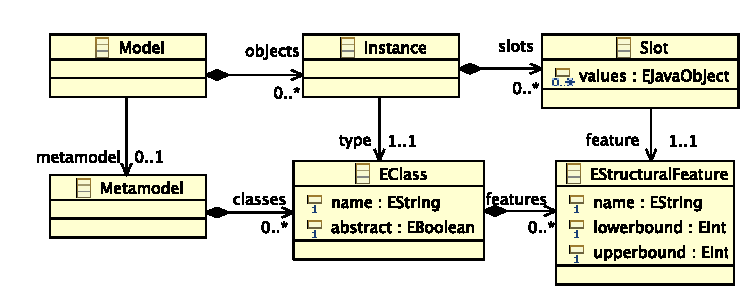
\includegraphics[scale=0.75]{5.Implementation/cope_mm.pdf}
  \caption[The metamodel-independent representation used by COPE]{Simplification of the metamodel-independent representation used by COPE, based on \cite{herrmannsdoerfer09cope}.}
  \label{fig:cope_mmi}
\end{figure}

Listing~\ref{lst:cope} shows the COPE model migration strategy for the Petri net example given above\footnote{In Listing~\ref{lst:cope}, some of the concrete syntax has been changed in the interest of readability.}. Most notably, slots for features that no longer exist must be explicitly \texttt{unset}. In Listing~\ref{lst:cope}, slots are \texttt{unset} on four occasions, once for each feature that exists in the original metamodel but not the evolved metamodel. Namely, these features are: \texttt{src} and \texttt{dst} of \texttt{Transition} and of \texttt{Place}. Failing to \texttt{unset} slots that do not conform with the evolved metamodel causes migration to fail with an error.

\begin{lstlisting}[caption=Petri nets model migration in COPE, label=lst:cope, language=COPE]
for (transition in Transition.allInstances) {
  for (source in transition.unset('src')) {
    def arc = petrinets.PTArc.newInstance()
    arc.src = source;  arc.dst = transition;
    arc.net = transition.net
  }

  for (destination in transition.unset('dst')) {
    def arc = petrinets.TPArc.newInstance() 
    arc.src = transition; arc.dst = destination;
    arc.net = transition.net
  }
}

for (place in Place.allInstances) {
  place.unset('src');  place.unset('dst');
}
\end{lstlisting}


\subsection{Requirements Identification}
\label{subsec:analysis}
By analysing existing approaches to managing developer-driven co-evolution, requirements were derived for a domain-specific language for specifying and executing model migration. The derivation of the requirements is now summarised, by considering two dimensions: the source-target relationship of the language used for specifying migration strategies and the way in which models are represented during migration. %and the structures provided by the language for specifying and re-using migration strategies.


\subsubsection{Source-Target Relationship}
New target transformation languages (Section \ref{subsubsec:m2m}) require code for explicitly copying from the original to the evolved metamodel those model elements that are unaffected by the metamodel evolution. In contrast, model migration strategies written in COPE (Section~\ref{subsubsec:cope}) must explicitly unset any data that is not to be copied from the original to the migrated model. The Ecore2Ecore approach (Section~\ref{subsubsec:ecore2ecore}) does not require explicit copying or unsetting code. Instead, the relationship between original and evolved metamodel elements is captured in a mapping model specified by the metamodel developer. The mapping model can be configured by hand or, in some cases, automatically derived. 

In each case, extra effort is required when defining a migration strategy due to the way in which the co-evolution approach relates source (original) and target (migrated) model elements. This observation led to the following requirement: \emph{The migration language must \textbf{automatically} copy every model element that conforms to the evolved metamodel from original to migrated model, and must not automatically copy any model element that does not conform to the evolved metamodel from original to migrated model.}


\subsubsection{Model Representation}
When using the Ecore2Ecore approach, model elements that do not conform to the evolved metamodel are accessed via XMI. Consequently, the metamodel developer must be familiar with XMI and must perform tasks such as dereferencing URI fragments (Listing~\ref{lst:java}) and type conversion. With COPE and the Epsilon Transformation Language, models are loaded using a modelling framework (and so migration strategies need not be concerned with the representation used to store models). Consequently, the following requirement was identified: \emph{The migration language must not expose the underlying representation of original or migrated models.}

To apply co-evolution operators, COPE requires the metamodel developer to use a specialised metamodel editor, which can manipulate only metamodels defined with EMF. Like, the Ecore2Ecore approach, COPE can be used only to manage co-evolution for models and metamodels specified with EMF. Tight coupling to EMF allows the Ecore2Ecore approach to schedule migration automatically, during model loading. To better support integration with modelling frameworks other than EMF, the following requirement was derived: \emph{The migration language must be loosely coupled with modelling frameworks and must not assume that models and metamodels will be represented in EMF.}


% \subsubsection{Re-use of migration strategies}
% To produce a suitable migration strategy, each approach requires some effort on the part of the metamodel developer during metamodel evolution. As we discuss more thoroughly in \cite{rose09analysis}, there is a trade-off between the amount of effort required and the flexibility of the approach. 
% 
% COPE seeks to reduce the effort required to express a migration strategy with co-evolutionary operators, which specify re-usable fragments of a migration strategy. With COPE, co-evolutionary operators are applied to perform metamodel evolution and later used to automatically generate a corresponding migration strategy. To apply co-evolution operators, COPE requires the metamodel developer to use a specialised metamodel editor and therefore it is not clear whether operator-based co-evolution can be used with all categories of metamodel editing tool, as we discuss more thoroughly in \cite{rose09analysis}.
% 
% The Ecore2Ecore approach and Epsilon Transformation Language do not require metamodel evolution to occur in a specialised editor and do not provide structures for specifying or re-using migration strategy fragments.
% 
% No existing approach investigates whether it is possible to provide re-usable migration strategy fragments without requiring a specialised metamodel editor. To explore this, the following requirements were derived:  \emph{Epsilon Flock must provide re-usable structures for expressing commonly occurring fragments of migration strategies. Application of the re-usable structures must not require a specialised metamodel editor.}